% !TeX spellcheck = hu_HU
% !TeX encoding = UTF-8

\chapter{Infrastruktúramenedzsment: Uyuni}
Nagyméretű informatikai infrastruktúra kezelése esetén elengedhetetlen valamiféle infrastruktúramenedzsment-eszköz használata. Ez nem csak könnyebbé teszi az üzemeltetést, de számos kiegészítő funkcióval is rendelkezik, lényegében egy helyen láthatunk minden releváns adatot, és egyazon felületről van lehetőségünk frissítések telepítésére és biztonsági sérülékenységek leírásainak böngészésre, mint ahol azt is tároljuk, hogy egy adott virtuális gép melyik gazdagépen fut, és az hol található.

Mivel ez a megoldás hasznosnak és érdekesnek tűnt számomra, és a dolgozat profiljába is jól illeszkedik, úgy döntöttem, hogy a tesztkörnyezet kezelésére is fogok ilyen megoldást alkalmazni. A választásom az Uyuni-ra esett, mely gyakorlatilag mindent tud, amire szükségem volt, és ingyenesen elérhető. A döntésben az is segített, hogy a projektet a SUSE támogatja, a fejlesztésében is részt vesz (az Uyuni szolgál a kereskedelmi forgalomban lévő SUSE Manager megoldás alapjául), és az openSUSE-alapú disztribúciókra is kiemelt figyelmet fordítanak, így nem kellett kompatibilitási problémákkal foglalkoznom. Az Uyuni a Salt konfigurációmenedzsment és automatizációs keretrendszerre épül, mely szintén széleskörűen használt és támogatott.


\section{Telepítés}
\label{sect:uyuni-install}
Az Uyuni meglehetősen erőforrás-igényes, a telepítéséhez minimum négy CPU-mag, 16~GB memória és  több száz gigabyte tárhely lehet szükséges a használni kívánt telepítőforrásoktól függően~\cite{UyuniInstallGuide}. Éles környezetben még ennél is több memóriát javasolnak, így az Uyuni számára létrehozott virtuális gép lett a környezet leginkább erőforrás-igényes rendszere, melynek telepítéshez használt parancs és a \acrshort{vm} leírója látható \aref{lst:virtinstall} és \aref{lst:virshxml} kódrészleteken. Ezeken megfigyelhetjük, hogy a virtuális gépet 12~CPU-maggal és 32~GB memóriával hoztam létre, a particionálásra a későbbiek folyamán fogok részletesen kitérni.

Ahogy a korábbiakban írtam, az Uyuni jó támogatottságnak örvend az openSUSE platformon. A telepítési kézikönyvben egy dedikált openSUSE Leap 15.5-ös \acrshort{os}-verziót futtató számítógépet javasolnak az infrastruktúramenedzsment-program telepítéséhez~\cite{UyuniInstallGuide}.
Ennek megfelelően én is ezt a verziót telepítettem, és bár a Leap alapértelmezett telepítési forrásaiban nem szerepel az Uyuni, de az ezt tartalmazó telepítőforrást egyetlen paranccsal felvehetjük, és ezt követően a segítségével telepíthetjük is az Uyunit.

\subsection{Kötetkiosztás}
A particionálás kérdése azért is kiemelt fontosságú az Uyuni telepítése során, mert a telepítés folyamán ezen feltételek meglétét ellenőrzi is a telepítő, és nem teljesülésük esetén a telepítés hibára futhat. A kötetek kiosztása során a hivatalos útmutatóból indultam ki, viszont a felhasználási célok figyelembevételével néhány partíciót a javasoltnál nagyobbra állítottam be, ennek megfelelően jött létre \aref{tab:uyuni-partitioning}.~táblázatban ismertetett felépítés. Elsősorban a spacewalk kötet növelése volt indokolt, hiszen az Uyuni egyik fontos része a szoftvercsomagok kezelése. Ennek gördülékeny és hatékony használatához a rendszer letükrözi a szükséges telepítőforrásokat, melyek jelentős helyigénnyel rendelkeznek, melyre \aref{sect:reposync} alfejezetben térek ki részletesen.

\begin{table}[h]
	\setlength{\tabcolsep}{5pt}
	\renewcommand{\arraystretch}{1.3}
	\centering
	\begin{tabular}{||l l l l m{5.3cm}||}
		\hline
		Kötet & Csatolási pont & Méret & Típus & Leírás\\
		\hline\hline
		boot & /boot & 1~GB & fizikai, ext4 & Az \acrshort{os} betöltéséhez szükséges fájlok tárhelye. \\
		\hline
		root & / & 40~GB & \acrshort{lvm}, XFS & A könyvtár-hierarchia legfelső eleme, a rendszerfájlok helye. \\
		\hline
		pgsql & /var/lib/pgsql & 52~GB & \acrshort{lvm}, XFS & A PostgreSQL adatbázismotor által tárolt adatok könyvtára. \\
		\hline
		spacewalk & /var/spacewalk & 100~GB & \acrshort{lvm}, XFS & Az infrastruktúramenedzsment\Hyphdash szoftver által használt fájlok elsődleges helye. \\
		\hline
		cache & /var/cache & 12~GB & \acrshort{lvm}, XFS & Gyorsítótárazott adatok könyvtára. \\
		\hline
		swap & swap & 4~GB & \acrshort{lvm}, swap & Virtuális memóriaként használt lemezterület. \\
		\hline
	\end{tabular}
	\caption{Az infrastruktúramenedzsment-szerver telepítéskori kötetkiosztása.}
	\label{tab:uyuni-partitioning}
\end{table}

\section{Telepítőforrások tükrözése}
\label{sect:reposync}
Ahogy az előző alfejezetben már említettem, az Uyuni egyik központi feladata a telepítőforrások és szoftvercsomagok kezelése a bevont rendszereken. Ehhez a használni kívánt telepítőforrásokat le kell tükröznünk az Uyunit futtató szerverre. Ez a megoldás elsőre túlzásnak tűnhet, hiszen egy-egy ilyen forrás több tíz, egyes esetekben több száz gigabyte lehet, azonban egy nagyméretű infrastruktúránál megvannak az előnyei. Gondoljunk csak bele, hogy mekkora hálózati forgalmat takaríthatunk meg azzal, hogy a telepítendő szoftverek és operációsrendszer-frissítések letöltésekor nem kell minden esetben az internetről letölteni a szükséges csomagokat, hanem ezt elegendő mindössze egyszer, az Uyuni szerveren megtenni, és onnantól kezdve az összes kliens már a belső hálózatról érheti el a szükséges programokat.
Emellett hasznos lehet egy offline példány megtartása is a telepített csomagokból, hiszen előfordulhat, hogy egy harmadik fél által üzemeltetett telepítési forrás elérhetetlenné válik, és így nem férünk hozzá a kívánt csomagokhoz.

Ahhoz, hogy egy-egy ilyen csomagtárhelyet letükrözhessünk, létre kell hozni úgynevezett \textit{Software Channel}-eket, melyek lényegében a repository-t csomagolják be egy magasabb szintű egységbe. Ez tárolja, hogy milyen csomagok érhetőek el, ezek milyen architektúrán használhatóak, lehetővé teszik a csomagforrások kezelését, és hozzárendelhetjük őket a kliensekhez. A csatornák által tartalmazott repository-k tárolják, hogy milyen címen érhető el a tükrözendő telepítőforrás, és hogy az adott repository melyik csatornához van hozzárendelve.

A tesztkörnyezethez is tükröztem telepítési forrásokat. Mivel a gépek többsége openSUSE Leap~15.5-ös verziót használt, ezért az ehhez tartozó csomagok szinkronizálásával kezdtem. Minden alapértelmezett forrást letükröztem, illetve az Uyuni általi menedzselés céljából az Uyuni-csomagokat tartalmazó repository-t is felvettem a szinkronizálandók közé. Az egyszerűbb kezelés miatt a csatornák hierarchiába szervezhetőek, így csak a kiválasztott szülőcsatornával (base channel) kompatibilis gyermekcsatornákat vehetünk fel egy adott klienshez. A tesztkörnyezetben létrehozott telepítőforrás-hierarchiát \aref{fig:software-channels}.~ábra szemlélteti.

\begin{figure}[ht]
	\centering
	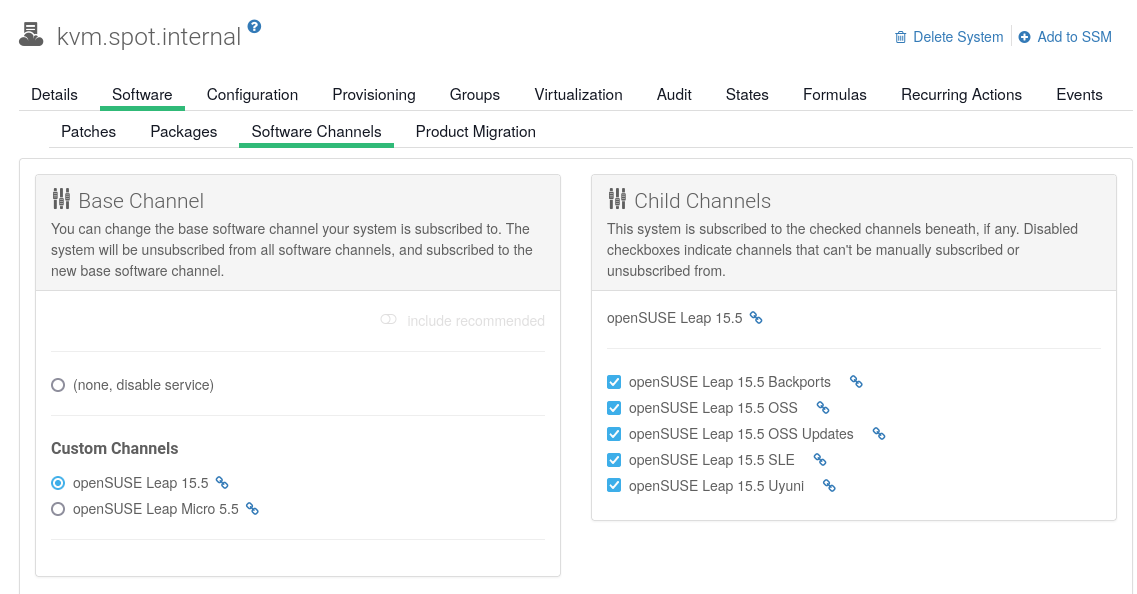
\includegraphics[width=15cm]{figures/uyuni-channels.png}
	\caption{A kialakított csatornahierarchia.}
	\label{fig:software-channels}
\end{figure}

Az első repository tükrözése a vártnál közel 20\%-kal több tárhelyet igényelt a spacewalk köteten (\ref{fig:reposync-disk-usage}.~ábra), így szükségessé vált a partíció megnövelése. Ennek megvalósításához az~\acrshort{lvm} által biztosított \texttt{lvextend} parancsot használtam, mely a logikai kötet megnövelésén túl a fájlrendszer (itt XFS) kiterjesztését is támogatja. Ez a parancs viszont csak akkor használható, ha a kötetcsoportban~(\acrshort{vg}) rendelkezésre áll annyi szabad hely, amennyivel bővíteni szeretnénk a tárhelyet. Mivel azonban itt ez a feltétel nem teljesült, több szinten kellett elvégezni a kötet megnövelését, először a~\acrshort{kvm}-hoszton kellett megnövelni a virtuális géphez tartozó tárterületet. További kihívást jelentett, hogy a kiterjesztést a~\acrshort{vm} leállítása nélkül szerettem volna elvégezni. Ebben az esetben nem jelentett volna nagy gondot a gép újraindítása, viszont szerettem volna felkészülni olyan helyzetekre is, amikor a gép leállítása nem megengedhető. Ilyen lehet például, ha a szinkronizálás alatt álló telepítőforrás a vártnál jelentősen nagyobb méretűnek bizonyul, vagy éppen a~PostgreSQL által használt tárhely van fogytán, de még nem fejeződött be a korábban indított indexelés. Mindezek mellett általában éles környezetben is korlátozottak a lehetőségeink egy-egy kiszolgáló újraindítására.

\begin{figure}[ht]
	\centering
	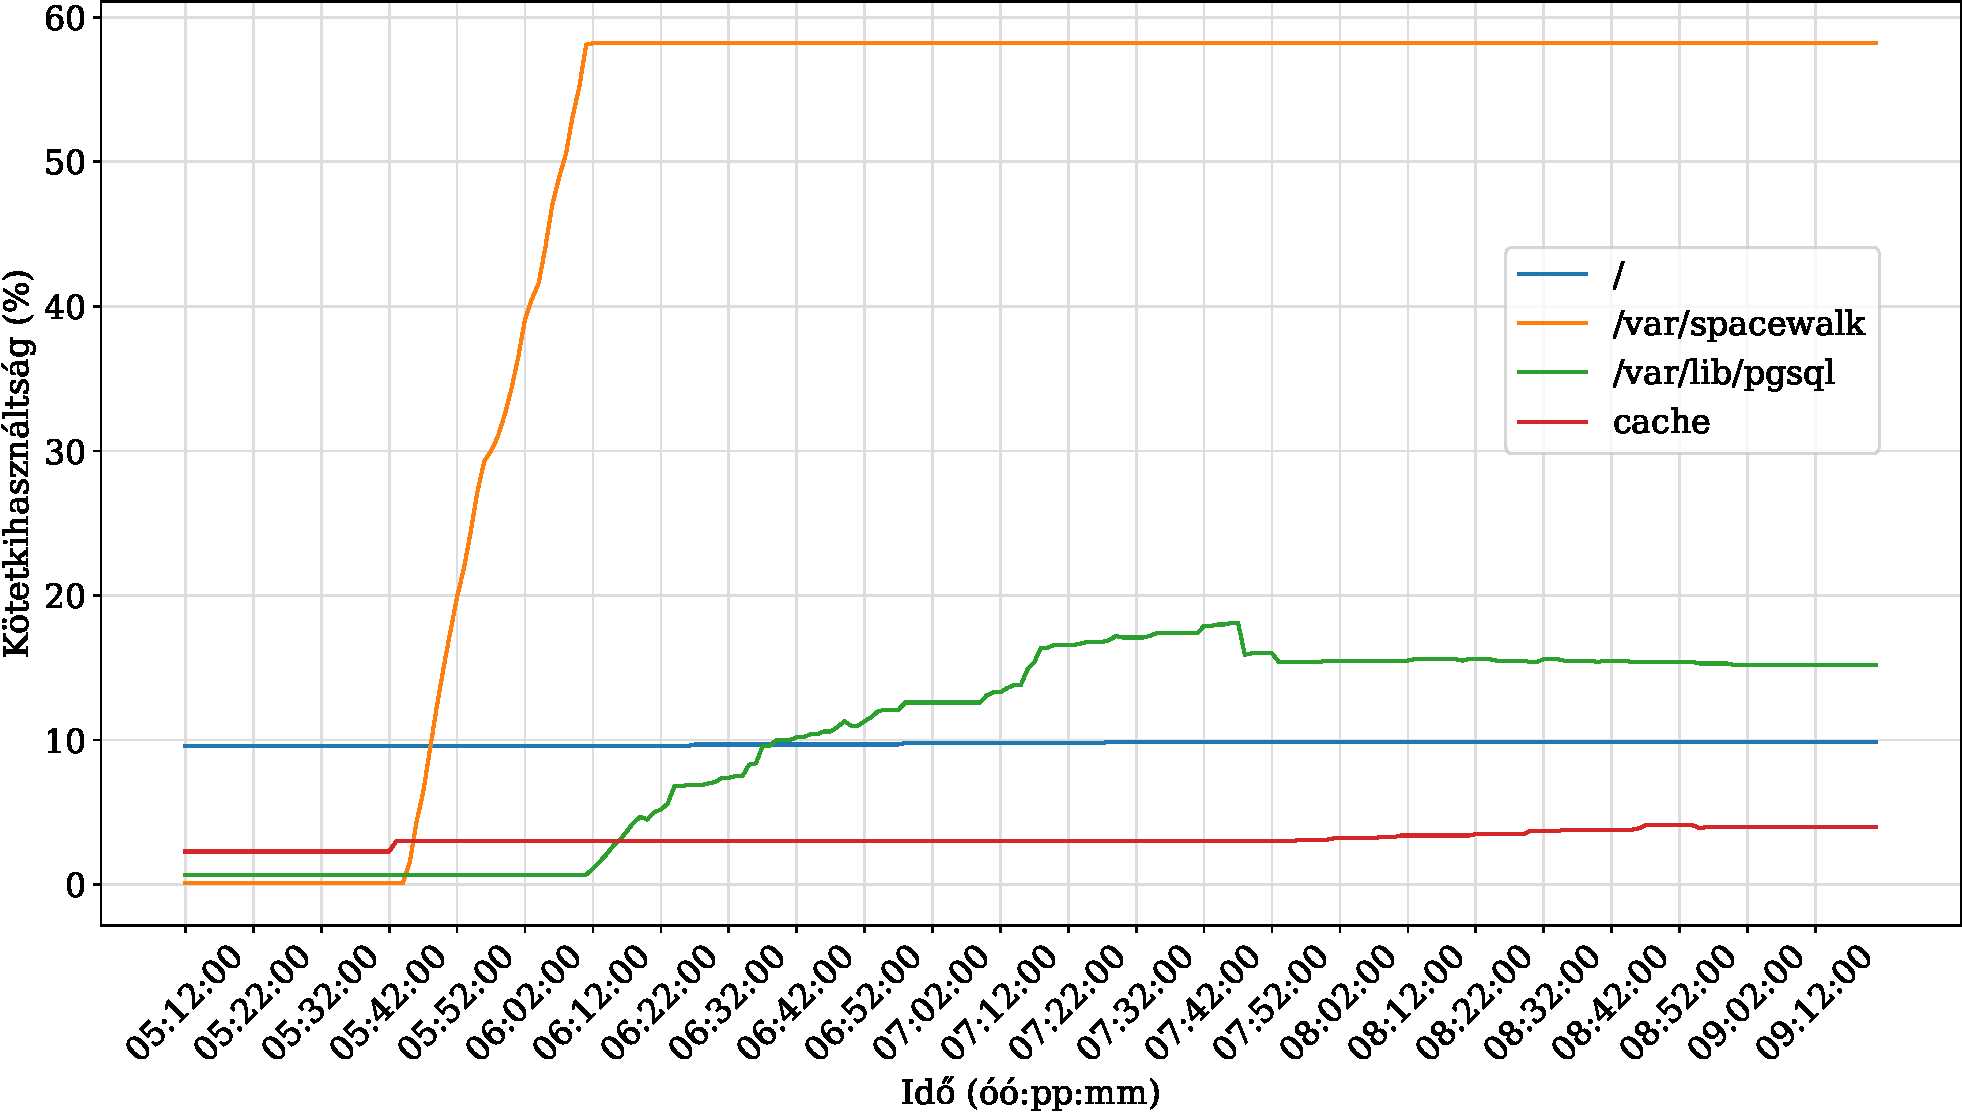
\includegraphics[width=15cm]{figures/reposync-leap-oss-disk-grid.pdf}
	\caption{Kötetkihasználtság változása az egyik telepítőforrás tükrözése során.}
	\label{fig:reposync-disk-usage}
\end{figure}

\subsection{Online kötetnövelés}
Ezen okokból a spacewalk kötet online megnövelése mellett döntöttem. Első lépésként a hosztgépen terjesztettem ki a virtuális gép számára fenntartott partíciót (a~\texttt{kvm-uyuni} logikai kötetet). \Aref{lst:virsh-blockresize}. kódrészleten látható, hogy ezt követően a virtuális gép még nem tudja használni a nagyobb méretű kötetet, szükséges még a \texttt{virsh blockresize} parancs futtatása, melynek hatására a virtuális gép számára is láthatóvá válik a nagyobb kötetméret. Ezt követően a~\acrshort{vm}-en növeltem meg a logikai kötetek alapjául szolgáló fizikai kötet~(\acrshort{pv}) méretét, melyet követően már a megszokott módon volt lehetőség a logikai kötet bővítésére.

\begin{lstlisting}[caption=Az infrastruktúramenedzsment-programokat futtató virtuális gép kötetének online megnövelése a gazdagépen.,label=lst:virsh-blockresize,escapechar=?]
	?\underline{10-151-7-5:$\sim$ \#}? virsh domblkinfo uyuni /dev/vg1/kvm-uyuni
	Capacity:       268435456000
	Allocation:     225145827328
	Physical:       375809638400
	?\underline{10-151-7-5:$\sim$ \#}? virsh blockresize uyuni --path /dev/vg1/kvm-uyuni --size 350G
	Block device '/dev/vg1/kvm-uyuni' is resized
	?\underline{10-151-7-5:$\sim$ \#}? virsh domblkinfo uyuni /dev/vg1/kvm-uyuni
	Capacity:       375809638400
	Allocation:     225145827328
	Physical:       375809638400
\end{lstlisting}
